\documentclass[a4paper,12pt]{article}
\usepackage[utf8]{inputenc}
\usepackage{graphicx}    % Para inserir imagens
\usepackage{amsmath}     % Para fórmulas matemáticas
\usepackage{amssymb}     % Para símbolos matemáticos
\usepackage{hyperref}    % Para links clicáveis
\usepackage{geometry}    % Para configurar margens
\usepackage{enumitem}    % Para listas personalizadas
\usepackage{caption}     % Para legendas de imagens e tabelas
\usepackage{float}       % Para melhor controlo da posição de imagens
\usepackage{titlesec}    % Para personalizar títulos das seções
\usepackage{array}
\usepackage{array}
\usepackage{makecell}
\usepackage{float}
\usepackage{array}     % Para customização de colunas
\usepackage{float}     % Para controlar a posição das tabelas
\usepackage{enumitem}  % Para listas personalizadas
\usepackage{multirow}
\usepackage{arydshln} % Coloca isso no preâmbulo


% Title, author, and date
\title{Spotify - Microservices Architecture}
\author{
    Aplicações na Web (AW) \\
    Group 22 \\[0.3cm]
    João Oliveira, fc56908 \\ 
    Sebastião Cancela, fc58282
}
\date{March 2025}

\begin{document}

\maketitle
\tableofcontents
\newpage

% Introduction section
\section{Introduction}

This document presents the architectural blueprint for a Spotify-inspired web application, designed to support a scalable, efficient, and modular system. The goal is to define a comprehensive architecture that encompasses both the back-end and front-end components, ensuring seamless interaction between services.

The blueprint will focus on designing a microservices-based backend, defining key resources, and establishing API communication. Additionally, it will outline the front-end architecture, including micro-front-ends, state management, and routing. Using an event-driven approach, the system will support real-time updates and scalable service orchestration.

This document serves as a technical reference, detailing the structural design choices necessary to build the application, ensuring maintainability, performance, and adaptability to future enhancements.

\begin{figure}[H]
    \centering
    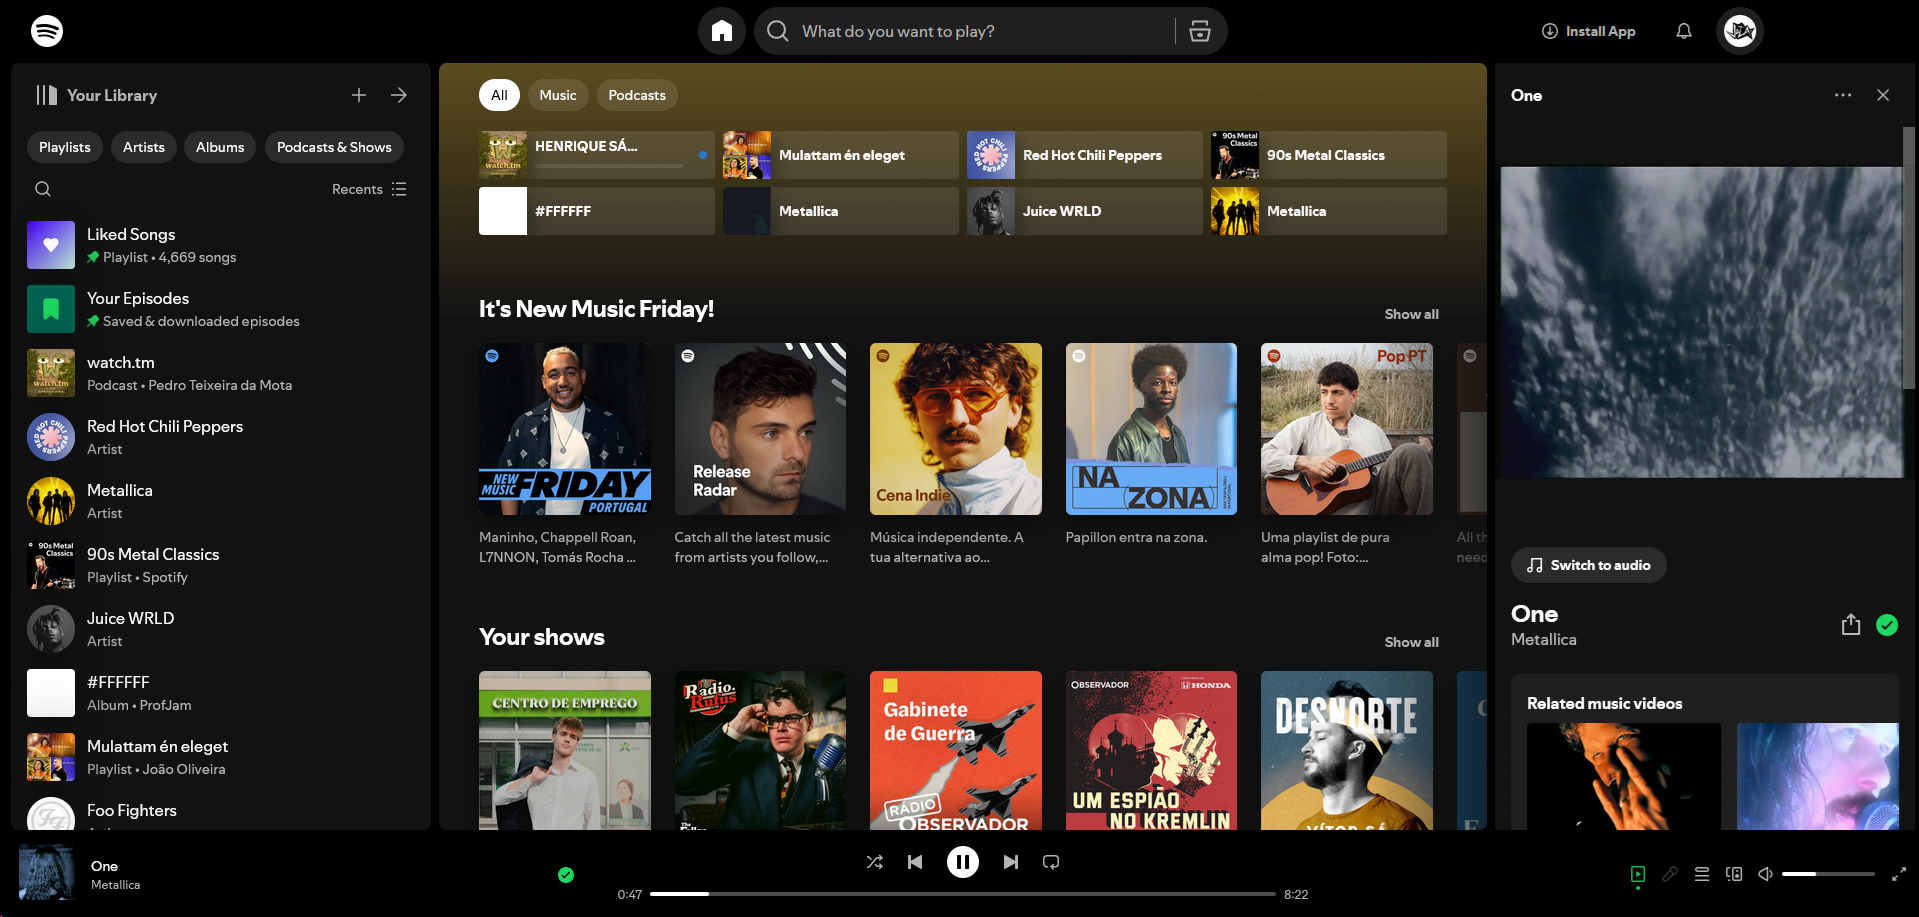
\includegraphics[width=\linewidth]{images/a.png}
    \caption{Spotify Web App}
    \label{fig:spotify-web-app}
\end{figure}


    \subsection{Current Phase Focus}
    This phase of the project focuses on the following core components:
    \begin{itemize}
        \item \textbf{Backend Services}: Identifying and defining the key backend services that support the core functionalities of the application.
        \item \textbf{Resources}: Specifying the resources managed by each service, including data entities and their relationships.
        \item \textbf{APIs}: Outlining the RESTful APIs that will enable interaction with the backend services.
        \item \textbf{Backend Orchestration}: Describing how services will communicate and coordinate to ensure smooth workflow execution across the system.
    \end{itemize}
    
    \subsection{Objective}
    The goal of this phase is to establish a solid architectural foundation that will support future development and ensure the system's scalability, maintainability, and efficiency.

\clearpage % Forces the next content to start on a new page

% BE Services section
\section{BE Services}
In this section, we define the back-end micro-services of this application.

% Auth Service
\begin{table}[H]
    \centering
    \renewcommand\arraystretch{1.5}
    \setlength{\tabcolsep}{5pt}
    \begin{tabular}{|>{\centering\arraybackslash}m{4cm}|m{10cm}|}
    \hline
    \textbf{BE Service and Description} & \textbf{Resource Description} \\
    \hline
    \textbf{Auth Service}: Manages user authentication, including login, signup, token management, and account verification. &
    \begin{itemize}[left=0pt]
        \item \textbf{UserCredential}: Stores essential user login information like email and password hash.  
        \item \textbf{AuthToken}: Token issued upon successful login, used to authenticate user requests.  
        \item \textbf{RefreshToken}: Token that allows users to renew their `AuthToken` without re-authenticating.  
        \item \textbf{VerificationToken}: Token used to verify user email addresses after registration. 
        \item \textbf{Session}: Stores active session information, including start and last activity timestamps.
    \end{itemize} \\
    \hline
    \end{tabular}
    \caption{Auth Service Overview with Managed Resources}
    \label{tab:auth-service}
\end{table}

% User Service
\begin{table}[H]
    \centering
    \renewcommand{\arraystretch}{1.5}
    \begin{tabular}{|>{\centering\arraybackslash}m{4cm}|m{10cm}|}
    \hline
    \textbf{BE Service and Description} & \textbf{Resource Description} \\
    \hline
    \textbf{User Service}: Manages user profiles, including personal information, preferences, and account status. & 
    \begin{itemize}[left=0pt]
        \item \textbf{User}: Contains users basic information like email and username.
        \item \textbf{Profile}: Contains users public information.
        \item \textbf{AccountStatus}: Indicates the current status of a user account.
        \item \textbf{Activity}: Tracks the user's recent interactions, such as played media and followed artists, for history and personalization purposes.
    \end{itemize} \\
    \hline
    \end{tabular}
    \caption{User Service Overview with Managed Resources}
    \label{tab:user-service}
\end{table}

% Media Service
\begin{table}[H]
    \centering
    \renewcommand{\arraystretch}{1.5}
    \begin{tabular}{|>{\centering\arraybackslash}m{4cm}|m{10cm}|}
    \hline
    \textbf{BE Service and Description} & \textbf{Resource Description} \\
    \hline
    \textbf{Media Service}: Manages all media content, including tracks, albums, podcasts, episodes, and audiobooks. Also handles playback, downloads, and playlists. & 
    \begin{itemize}[left=0pt]
        \item \textbf{Artist}: Represents music artists with attributes like artist\_id, name, bio, genre, image\_url.
        \item \textbf{Track}: Attributes include title, duration, artist ID, and audio URL.
        \item \textbf{Album}: Contains multiple tracks with attributes like title, release date, and artist ID.
        \item \textbf{Podcast}: Contains podcast metadata like title, description, host, and release date.
        \item \textbf{Episode}: Attributes include episode ID, title, duration, audio URL, and release date.
        \item \textbf{Playlist}: User-created playlists with title, description, and a list of tracks.
        \item \textbf{PlaybackSession}: Represents playback status with attributes like progress, status, and media ID.
        \item \textbf{Favorite}: Adds the media to the users library.
        \item \textbf{Follow}: Manages relationships where users follow artists or podcasts.
    \end{itemize} \\
    \hline
    \end{tabular}
    \caption{Media Service Overview with Managed Resources}
\end{table}

% Search Service
\begin{table}[H]
    \centering
    \renewcommand{\arraystretch}{1.5}
    \begin{tabular}{|>{\centering\arraybackslash}m{4cm}|m{10cm}|}
    \hline
    \textbf{BE Service and Description} & \textbf{Resource Description} \\
    \hline
    \textbf{Search Service}: Provides search functionality across media, artists, and playlists. & 
    \begin{itemize}[left=0pt]
        \item \textbf{SearchQuery}: Captures user search input and filters.
    \end{itemize} \\
    \hline
    \end{tabular}
    \caption{Search Service Overview with Managed Resources}
\end{table}

% Notification Service
\begin{table}[H]
    \centering
    \renewcommand{\arraystretch}{1.5}
    \begin{tabular}{|>{\centering\arraybackslash}m{4cm}|m{10cm}|}
    \hline
    \textbf{BE Service and Description} & \textbf{Resource Description} \\
    \hline
    \textbf{Notification Service}: Manages notifications for new releases and updates related to followed media and artists. &
    \begin{itemize}[left=0pt]
        \item \textbf{Notification}: Represents a notification sent to the user, including content, type (new release, update), and timestamp.
    \end{itemize} \\
    \hline
    \end{tabular}
    \caption{Notification Service Overview with Managed Resources}
\end{table}

% Recommendation Service
\begin{table}[H]
    \centering
    \renewcommand{\arraystretch}{1.5}
    \begin{tabular}{|>{\centering\arraybackslash}m{4cm}|m{10cm}|}
    \hline
    \textbf{BE Service and Description} & \textbf{Resource Description} \\
    \hline
    \textbf{Suggest Service}: Provides personalized suggestions for users based on their activity, listening habits, and trending content. &
    \begin{itemize}[left=0pt]
        \item \textbf{Suggestion}: Stores and manages recommended content for users, such as suggested tracks, albums, artists, and playlists.
    \end{itemize} \\
    \hline
    \end{tabular}
    \caption{Suggest Service Overview with Managed Resources}
\end{table}

 \clearpage

% Resources section
\section{Resources}
Each back-end service manages a specific set of resources. 

% Auth Resources
\begin{table}[H]
    \centering
    \renewcommand{\arraystretch}{1.2}
    \setlength{\tabcolsep}{5pt}
    \begin{tabular}{|>{\centering\arraybackslash}m{5.5cm}|m{2.5cm}|m{6.0cm}|}
    \hline
    \textbf{BE Services} & \textbf{Operations} & \textbf{Endpoints} \\
    \hline
    \multirow{7}{*}{\textbf{Auth Service}} 
        & POST & /auth/login \\
        & POST & /auth/refresh \\
        & POST & /auth/verify \\
        & DELETE & /auth/logout \\
        \cdashline{2-3}        
        & GET & /auth/sessions \\
        & GET & /auth/sessions/\{session\_id\} \\
        & DELETE & /auth/sessions/\{session\_id\} \\
    \hline
    \end{tabular}
    \caption{Auth Service Operations and Endpoints}
\end{table}

% User Resources
\begin{table}[H]
    \centering
    \renewcommand{\arraystretch}{1.2}
    \begin{tabular}{|>{\centering\arraybackslash}m{5.5cm}|m{2.5cm}|m{6.0cm}|}
    \hline
    \textbf{BE Services} & \textbf{Operations} & \textbf{Endpoints} \\
    \hline
    \multirow{12}{*}{\textbf{User Service}} 
        & POST & /users \\ % Create user account 
        & PUT & /users/\{user\_id\} \\ % Edit user data
        & DELETE & /users/\{user\_id\} \\ % Delete users account
        \cdashline{2-3}
        & GET & /users/me \\ % Get private data of the authenticated user
        \cdashline{2-3}
        & GET & /users/\{user\_id\}/profile \\ % Get user's public profile
        & PUT & /users/\{user\_id\}/profile \\ % Update user's public profile
        \cdashline{2-3}
        & GET & /users/me/following \\ % List of users/artists/podcasts followed by authenticated user
        & GET & /users/\{user\_id\}/following \\ % List of users the user follows
        & GET & /users/\{user\_id\}/followers \\ % List of users that follow the user
        & PUT & /users/me/following \\ % Update the list of followed users
        \cdashline{2-3}
        & GET & /users/\{user\_id\}/status \\ % Get account status
        & PUT & /users/\{user\_id\}/status \\ % Update account status
        \cdashline{2-3}
        & GET & /users/\{user\_id\}/activity \\ % Get user activity history
    \hline
    \end{tabular}
    \caption{User Service Operations and Endpoints}
\end{table}

% Media Resources (Tracks & Albums)
\begin{table}[H]
    \centering
    \renewcommand{\arraystretch}{1.2}
    \begin{tabular}{|>{\centering\arraybackslash}m{4.0cm}|m{2.5cm}|m{7.5cm}|}
    \hline
    \textbf{BE Services} & \textbf{Operations} & \textbf{Endpoints} \\
    \hline
    \multirow{12}{*}{\makecell{\textbf{Media Service} \\ Tracks \& Albums}}
        & POST & /tracks \\
        & GET & /tracks \\
        & GET & /tracks/\{track\_id\} \\
        & PUT & /tracks/\{track\_id\} \\ % Atualizar track
        & DELETE & /tracks/\{track\_id\} \\
        \cdashline{2-3}
        & POST & /albums \\ % Criar álbum
        & GET & /albums/\{album\_id\} \\
        & PUT & /albums/\{album\_id\} \\ % Atualizar álbum
        & DELETE & /albums/\{album\_id\} \\ % Apagar álbum
        \cdashline{2-3}
        & POST   & /albums/\{album\_id\}/tracks \\ % Adicionar música ao álbum
        & GET    & /albums/\{album\_id\}/tracks \\ % Listar músicas do álbum
        & DELETE & /albums/\{album\_id\}/tracks/\{track\_id\} \\ % Remover música do álbum
    \hline
    \end{tabular}
    \caption{Media Service - Tracks \& Albums}
\end{table}

% Media Resources (Artists & Podcasts)
\begin{table}[H]
    \centering
    \renewcommand{\arraystretch}{1.2}
    \begin{tabular}{|>{\centering\arraybackslash}m{4.0cm}|m{2.5cm}|m{7.5cm}|}
    \hline
    \textbf{BE Services} & \textbf{Operations} & \textbf{Endpoints} \\
    \hline
    \multirow{9}{*}{\makecell{\textbf{Media Service} \\ Artists \& Podcasts}} 
        & POST & /artists \\
        & GET & /artists \\
        & GET & /artists/\{artist\_id\} \\
        & PUT & /artists/\{artist\_id\} \\ % Atualizar perfil do artista
        & GET    & /artists/\{artist\_id\}/tracks \\ % Listar músicas do artista
        & POST   & /artists/\{artist\_id\}/tracks \\ % Adicionar música ao artista (opcional)
        & DELETE & /artists/\{artist\_id\}/tracks/\{track\_id\} \\ % Remover música do artista
        \cdashline{2-3}
        & POST & /podcasts \\ % Criar podcast
        & GET & /podcasts \\ % ver podcasts
        & GET & /podcasts/\{podcast\_id\} \\
        & PUT & /podcasts/\{podcast\_id\} \\ % Atualizar podcast
        & DELETE & /podcasts/\{podcast\_id\} \\ % Apagar podcast
        \cdashline{2-3}        
        & GET & /podcasts/\{podcast\_id\}/episodes \\
        & PUT & /podcasts/\{podcast\_id\}/episodes \\ % Atualizar podcast
    \hline
    \end{tabular}
    \caption{Media Service - Artists \& Podcasts}
\end{table}

% Media Resources (Episodes & Playlists)
\begin{table}[H]
    \centering
    \renewcommand{\arraystretch}{1.2}
    \begin{tabular}{|>{\centering\arraybackslash}m{4.0cm}|m{2.5cm}|m{7.5cm}|}
    \hline
    \textbf{BE Services} & \textbf{Operations} & \textbf{Endpoints} \\
    \hline
    \multirow{13}{*}{\makecell{\textbf{Media Service} \\ Episodes \& Playlists}} 
        & POST & /episodes \\ % Criar episódio
        & GET & /episodes/\{episode\_id\} \\
        & PUT & /episodes/\{episode\_id\} \\ % Atualizar episódio
        & DELETE & /episodes/\{episode\_id\} \\ % Apagar episódio
        \cdashline{2-3}
        & POST & /playlists \\
        & GET & /playlists \\
        & GET & /playlists/\{playlist\_id\} \\
        & PUT & /playlists/\{playlist\_id\} \\ % Atualizar nome/descrição da playlist
        & DELETE & /playlists/\{playlist\_id\} \\
        \cdashline{2-3}
        & POST & /playlists/\{playlist\_id\}/tracks \\ % addd track to playlist
        & GET & /playlists/\{playlist\_id\}/tracks \\ % addd track to playlist
        & PUT & /playlists/\{playlist\_id\}/tracks \\ % Atualizar a ordem das faixas
        & DELETE & /playlists/\{playlist\_id\}/tracks/\{track\_id\} \\ % addd track to playlist
    \hline
    \end{tabular}
    \caption{Media Service - Episodes \& Playlists}
\end{table}

% Media Resources (Playback & Queue)
\begin{table}[H]
    \centering
    \renewcommand{\arraystretch}{1.2}
    \begin{tabular}{|>{\centering\arraybackslash}m{4.0cm}|m{2.5cm}|m{7.5cm}|}
    \hline
    \textbf{BE Services} & \textbf{Operations} & \textbf{Endpoints} \\
    \hline
    \multirow{11}{*}{\makecell{\textbf{Media Service} \\ Playback \& Queue}} 
        & GET & /playback \\
        & POST & /playback/resume \\ % Pular para a próxima música
        & POST & /playback/stop \\ % Voltar para a música anterior
        & POST & /playback/play/\{media\_id\} \\ % Pular para a próxima música
        & POST & /playback/previous \\ % Voltar para a música anterior
        & POST & /playback/next \\ % Pular para a próxima música
        & POST & /playback/previous \\ % Voltar para a música anterior
        & PUT & /playback/shuffle \\
        & PUT & /playback/repeat \\
        \cdashline{2-3}
        & GET & /queue \\
        & DELETE & /queue \\ % Remover da fila
        & PUT & /queue/order \\
        & POST & /queue/tracks/\{track\_id\} \\ % Adicionar à fila
        & DELETE & /queue/tracks/\{track\_id\} \\ % Remover da fila
    \hline
    \end{tabular}
    \caption{Media Service - Playback \& Queue}
\end{table}

% Media Resources (Favorites & Follows)
\begin{table}[H]
    \centering
    \renewcommand{\arraystretch}{1.2}
    \begin{tabular}{|>{\centering\arraybackslash}m{4.0cm}|m{2.5cm}|m{7.5cm}|}
    \hline
    \textbf{BE Services} & \textbf{Operations} & \textbf{Endpoints} \\
    \hline
    \multirow{10}{*}{\makecell{\textbf{Media Service} \\ Favorites \& Follows}} 
        & GET & /favorites \\
        & POST & /favorites/\{media\_id\} \\ % Adicionar aos favoritos
        & DELETE & /favorites/\{media\_id\} \\ % Remover dos favoritos
        \cdashline{2-3}
        & GET & /follows \\
        & GET & /follows/artists \\
        & POST & /follows/artists/\{artist\_id\} \\ % Seguir artista
        & DELETE & /follows/artists/\{artist\_id\} \\ % Deixar de seguir artista
        & GET & /follows/podcasts \\
        & POST & /follows/podcasts/\{podcast\_id\} \\ % Seguir artista
        & DELETE & /follows/podcasts/\{podcast\_id\} \\ % Deixar de seguir artista
    \hline
    \end{tabular}
    \caption{Media Service - Favorites \& Follows}
\end{table}


% Search Resources
\begin{table}[H]
    \centering
    \renewcommand{\arraystretch}{1.2}
    \begin{tabular}{|>{\centering\arraybackslash}m{4.0cm}|m{2.5cm}|m{7.5cm}|}
    \hline
    \textbf{BE Services} & \textbf{Operations} & \textbf{Endpoints} \\
    \hline
    \multirow{5}{*}{\textbf{Search Service}} 
        & GET & /search?q=\{query\}\&type=\{type\} \\
        & GET & /search/tracks?q=\{query\} \\
        & GET & /search/albums?q=\{query\} \\
        & GET & /search/artists?q=\{query\} \\
        & GET & /search/playlists?q=\{query\} \\
    \hline
    \end{tabular}
    \caption{Search Service Operations and Endpoints}
\end{table}

% Notification Resources
\begin{table}[H]
    \centering
    \renewcommand{\arraystretch}{1.2}
    \begin{tabular}{|>{\centering\arraybackslash}m{4.0cm}|m{2.5cm}|m{7.5cm}|}
    \hline
    \textbf{BE Services} & \textbf{Operations} & \textbf{Endpoints} \\
    \hline
    \multirow{1}{*}{\textbf{Notification Service}} 
    & GET & /notifications \\
    \hline
    \end{tabular}
    \caption{Notification Service Operations and Endpoints}
\end{table}

% Suggest Resources
\begin{table}[H]
    \centering
    \renewcommand{\arraystretch}{1.2}
    \setlength{\tabcolsep}{5pt}
    \begin{tabular}{|>{\centering\arraybackslash}m{4.0cm}|m{2.5cm}|m{7.5cm}|}
    \hline
    \textbf{BE Services} & \textbf{Operations} & \textbf{Endpoints} \\
    \hline
    \multirow{7}{*}{\textbf{Suggest Service}} 
    & GET & /suggestions \\
    & GET & /suggestions/new-releases \\
    & GET & /suggestions/made-for-you \\
    & GET & /suggestions/for-followers \\
    & GET & /suggestions/popular \\
    & GET & /suggestions/mood-based \\
    & GET & /suggestions/similar-to/\{track\_id\} \\
    \hline
    \end{tabular}
    \caption{Suggest Service Operations and Endpoints}
\end{table}

\clearpage % Forces the next content to start on a new page

\section{APIs}
Cada serviço expõe um conjunto de APIs RESTful para manipulação dos recursos.

\subsection{Exemplo de Endpoints para o Favorite Service}
\begin{itemize}
    \item \textbf{POST} \texttt{/favorites} – Adiciona um novo item aos favoritos.
    \item \textbf{DELETE} \texttt{/favorites/\{item\_id\}} – Remove um item dos favoritos.
    \item \textbf{GET} \texttt{/favorites} – Lista todos os favoritos de um utilizador.
\end{itemize}

\clearpage % Forces the next content to start on a new page

\section{BE Orchestration}
Esta seção detalha como os serviços de backend interagem entre si.

\subsection{Exemplo de Orquestração}
\begin{enumerate}
    \item O utilizador faz login via o \textbf{Auth Service}.
    \item Após autenticação, o \textbf{Favorite Service} é utilizado para listar músicas favoritas.
    \item O \textbf{Music Service} valida se cada música existe e se está ativa.
\end{enumerate}

\subsection{Fluxo de Exemplo}
\begin{enumerate}
    \item \textbf{Step 1}: Utilizador chama \texttt{POST /login} → `Auth Service`.  
    \item \textbf{Step 2}: Se autenticado, chama \texttt{GET /favorites} → `Favorite Service`.  
    \item \textbf{Step 3}: Para cada \texttt{item\_id}, o sistema verifica no \texttt{Music Service} se o conteúdo está disponível.  
\end{enumerate}

\end{document}